\begin{singlespace}
    \chapter{\textbf{Appendix D: Supplemental material for "Optimal resource investment to photosynthetic capacity maximizes nutrient allocation to whole plant growth under elevated CO$_2$"}}
\end{singlespace}

\setcounter{table}{0}
\renewcommand{\thetable}{D\arabic{table}}
\setcounter{figure}{0}
\renewcommand{\thefigure}{D\arabic{figure}}

\begin{table}[!h]
    \caption[Summary table containing volumes of compounds used to create modified Hoagland’s solutions for each soil nitrogen fertilization treatment]{Summary table containing volumes of compounds used to create modified Hoagland’s solutions for each soil nitrogen fertilization treatment. All volumes are expressed as milliliters per liter (mL L$^{-1}$)}
    \label{table:tab.d1}
    \resizebox{\columnwidth}{!}{
    \begin{tabular}{p{2.805cm}p{2cm}p{2cm}p{2cm}p{2cm}p{2cm}}
        \hline
        \textbf{Compound}
        & \multicolumn{1}{r}{\textbf{0 ppm N}}
        & \multicolumn{1}{r}{\textbf{35 ppm N}}
        & \multicolumn{1}{r}{\textbf{70 ppm N}}
        & \multicolumn{1}{r}{\textbf{105 ppm N}}
        & \multicolumn{1}{r}{\textbf{140 ppm N}} \\
        \hline
        1 M NH$_4$H$_2$PO$_4$   & \multicolumn{1}{r}{0}         & \multicolumn{1}{r}{0.165}     & \multicolumn{1}{r}{0.33}      & \multicolumn{1}{r}{0.5}       & \multicolumn{1}{r}{0.67} \\
        2 M KNO$_3$             & \multicolumn{1}{r}{0}         & \multicolumn{1}{r}{0.335}     & \multicolumn{1}{r}{0.67}      & \multicolumn{1}{r}{1}         & \multicolumn{1}{r}{1.33} \\
        2 M Ca(NO$_3$)$_2$      & \multicolumn{1}{r}{0}         & \multicolumn{1}{r}{0.335}     & \multicolumn{1}{r}{0.67}      & \multicolumn{1}{r}{1}         & \multicolumn{1}{r}{1.33} \\
        1 M NH$_4$NO$_3$        & \multicolumn{1}{r}{0}         & \multicolumn{1}{r}{0.165}     & \multicolumn{1}{r}{0.33}      & \multicolumn{1}{r}{0.5}       & \multicolumn{1}{r}{0.67} \\
        8 M NH$_4$NO$_3$        & \multicolumn{1}{r}{0}         & \multicolumn{1}{r}{0}         & \multicolumn{1}{r}{0}         & \multicolumn{1}{r}{0}         & \multicolumn{1}{r}{0} \\
        1 M KH$_2$PO$_4$        & \multicolumn{1}{r}{1}         & \multicolumn{1}{r}{0.85}      & \multicolumn{1}{r}{0.67}      & \multicolumn{1}{r}{0.5}       & \multicolumn{1}{r}{0.33} \\
        1 M KCl                 & \multicolumn{1}{r}{3}         & \multicolumn{1}{r}{2.45}      & \multicolumn{1}{r}{2}         & \multicolumn{1}{r}{1.5}       & \multicolumn{1}{r}{1} \\
        1 M CaCO$_3$            & \multicolumn{1}{r}{4}         & \multicolumn{1}{r}{3.33}      & \multicolumn{1}{r}{2.67}      & \multicolumn{1}{r}{2}         & \multicolumn{1}{r}{1.33} \\
        2 M MgSO$_4$            & \multicolumn{1}{r}{1}         & \multicolumn{1}{r}{1}         & \multicolumn{1}{r}{1}         & \multicolumn{1}{r}{1}         & \multicolumn{1}{r}{1} \\
        10\% Fe-EDTA            & \multicolumn{1}{r}{1}         & \multicolumn{1}{r}{1}         & \multicolumn{1}{r}{1}         & \multicolumn{1}{r}{1}         & \multicolumn{1}{r}{1} \\
        Trace elements          & \multicolumn{1}{r}{1}         & \multicolumn{1}{r}{1}         & \multicolumn{1}{r}{1}         & \multicolumn{1}{r}{1}         & \multicolumn{1}{r}{1} \\
        \hline
        &&&&&
        \\
        \hline
        \textbf{Compound}
        & \multicolumn{1}{r}{\textbf{210 ppm N}}
        & \multicolumn{1}{r}{\textbf{280 ppm N}}
        & \multicolumn{1}{r}{\textbf{350 ppm N}}
        & \multicolumn{1}{r}{\textbf{630 ppm N}} &
        \\
        \hline
        1 M NH$_4$H$_2$PO$_4$   & \multicolumn{1}{r}{1}         & \multicolumn{1}{r}{1}         & \multicolumn{1}{r}{1}         & \multicolumn{1}{r}{1}         &   \\
        2 M KNO$_3$             & \multicolumn{1}{r}{2}         & \multicolumn{1}{r}{2}         & \multicolumn{1}{r}{2}         & \multicolumn{1}{r}{2}         &   \\
        2 M Ca(NO$_3$)$_2$      & \multicolumn{1}{r}{2}         & \multicolumn{1}{r}{2}         & \multicolumn{1}{r}{2}         & \multicolumn{1}{r}{2}         &   \\
        1 M NH$_4$NO$_3$        & \multicolumn{1}{r}{1}         & \multicolumn{1}{r}{3.5}       & \multicolumn{1}{r}{0}         & \multicolumn{1}{r}{0}         &   \\
        8 M NH$_4$NO$_3$        & \multicolumn{1}{r}{0}         & \multicolumn{1}{r}{0}         & \multicolumn{1}{r}{0.75}      & \multicolumn{1}{r}{2}         &      \\
        1 M KH$_2$PO$_4$        & \multicolumn{1}{r}{0}         & \multicolumn{1}{r}{0}         & \multicolumn{1}{r}{0}         & \multicolumn{1}{r}{0}         &   \\
        1 M KCl                 & \multicolumn{1}{r}{0}         & \multicolumn{1}{r}{0}         & \multicolumn{1}{r}{0}         & \multicolumn{1}{r}{0}         &   \\
        1 M CaCO$_3$            & \multicolumn{1}{r}{0}         & \multicolumn{1}{r}{0}         & \multicolumn{1}{r}{0}         & \multicolumn{1}{r}{0}         &   \\
        2 M MgSO$_4$            & \multicolumn{1}{r}{1}         & \multicolumn{1}{r}{1}         & \multicolumn{1}{r}{1}         & \multicolumn{1}{r}{1}         &   \\
        10\% Fe-EDTA            & \multicolumn{1}{r}{1}         & \multicolumn{1}{r}{1}         & \multicolumn{1}{r}{1}         & \multicolumn{1}{r}{1}         &   \\
        Trace elements          & \multicolumn{1}{r}{1}         & \multicolumn{1}{r}{1}         & \multicolumn{1}{r}{1}         & \multicolumn{1}{r}{1}         &   \\
        \hline
\end{tabular}}
\end{table}
\clearpage

\newpage
\begin{table}[]
    \centering
    \caption{Summary of the daily growth chamber growing condition program}
    \label{table:tab.d2}
    %\resizebox{\columnwidth}{!}{%
    \begin{tabular}{|p{2cm}|p{4.5cm}|p{2cm}|}
        \hline
        Time  & Air temperature ($^{\circ}$C)   & Light (\%) \\
        \hline
        09:00 & \multirow{2}{*}{21}             & 25         \\
        09:45 &                                 & 50         \\
        \hline
        10:30 & \multirow{2}{*}{25}             & 75         \\
        11:15 &                                 & 100        \\
        \hline
        22:45 & \multirow{2}{*}{21}             & 75         \\
        23:30 &                                 & 50         \\
        \hline
        00:15 & \multirow{2}{*}{17}             & 25         \\
        01:00 &                                 & 0          \\
        \hline      
    \end{tabular}%}
\end{table}
\clearpage

\begin{table}[]
    \centering
    \caption[Effects of CO$_2$, fertilization, and inoculation on whole plant biomass: pot volume]{Effects of CO$_2$, fertilization, and inoculation on whole plant biomass: pot volume (BVR; g L$^{-1}$)$^*$}
    \label{table:tab.d3}
    %\resizebox{\columnwidth}{!}{
        \begin{tabular}{p{3.5cm}p{0.5cm}p{1.75cm}p{1.5cm}p{1.5cm}}
            \hline
            & \multicolumn{1}{r}{df} & \multicolumn{1}{r}{Coefficient}    & \multicolumn{1}{r}{$\chi^2$}  & \multicolumn{1}{r}{\textit{p}}
            \\
            \hline
    (Intercept)       & \multicolumn{1}{r}{-}       & \multicolumn{1}{r}{1.33E$-$01}    & \multicolumn{1}{r}{-}         & \multicolumn{1}{r}{-}               \\
    CO$_2$               & \multicolumn{1}{r}{1}    & \multicolumn{1}{r}{1.53E$-$01}    & \multicolumn{1}{r}{146.004}   & \multicolumn{1}{r}{\textbf{<0.001}} \\
    Inoculation (I)   & \multicolumn{1}{r}{1}       & \multicolumn{1}{r}{4.19E$-$01}    & \multicolumn{1}{r}{19.320}    & \multicolumn{1}{r}{\textbf{<0.001}} \\
    Fertilization (N) & \multicolumn{1}{r}{1}       & \multicolumn{1}{r}{1.90E$-$03}    & \multicolumn{1}{r}{279.387}   & \multicolumn{1}{r}{\textbf{<0.001}} \\
    CO$_2$*I             & \multicolumn{1}{r}{1}    & \multicolumn{1}{r}{1.03E$-$01}    & \multicolumn{1}{r}{0.007}     & \multicolumn{1}{r}{0.934}           \\
    CO$_2$*N             & \multicolumn{1}{r}{1}    & \multicolumn{1}{r}{2.44E$-$03}    & \multicolumn{1}{r}{49.725}    & \multicolumn{1}{r}{\textbf{<0.001}} \\
    I*N               & \multicolumn{1}{r}{1}       & \multicolumn{1}{r}{-6.90E$-$04}   & \multicolumn{1}{r}{9.006}     & \multicolumn{1}{r}{\textbf{0.003}}  \\
    CO$_2$*I*N           & \multicolumn{1}{r}{1}    & \multicolumn{1}{r}{-4.95E$-$04}   & \multicolumn{1}{r}{0.640}     & \multicolumn{1}{r}{0.424} \\
    \hline
    \end{tabular}%}
\end{table}
\begin{singlespace}
    \noindent \textsuperscript{$*$}Significance determined using Type II Wald $\chi^2$ tests ($\alpha$=0.05). \textit{P}-values less than 0.05 are in bold. Key: df=degrees of freedom; $\chi^2$=Wald Type II chi-square test statistic.
\end{singlespace}
\clearpage

\newpage
\begin{figure}
    \centering
    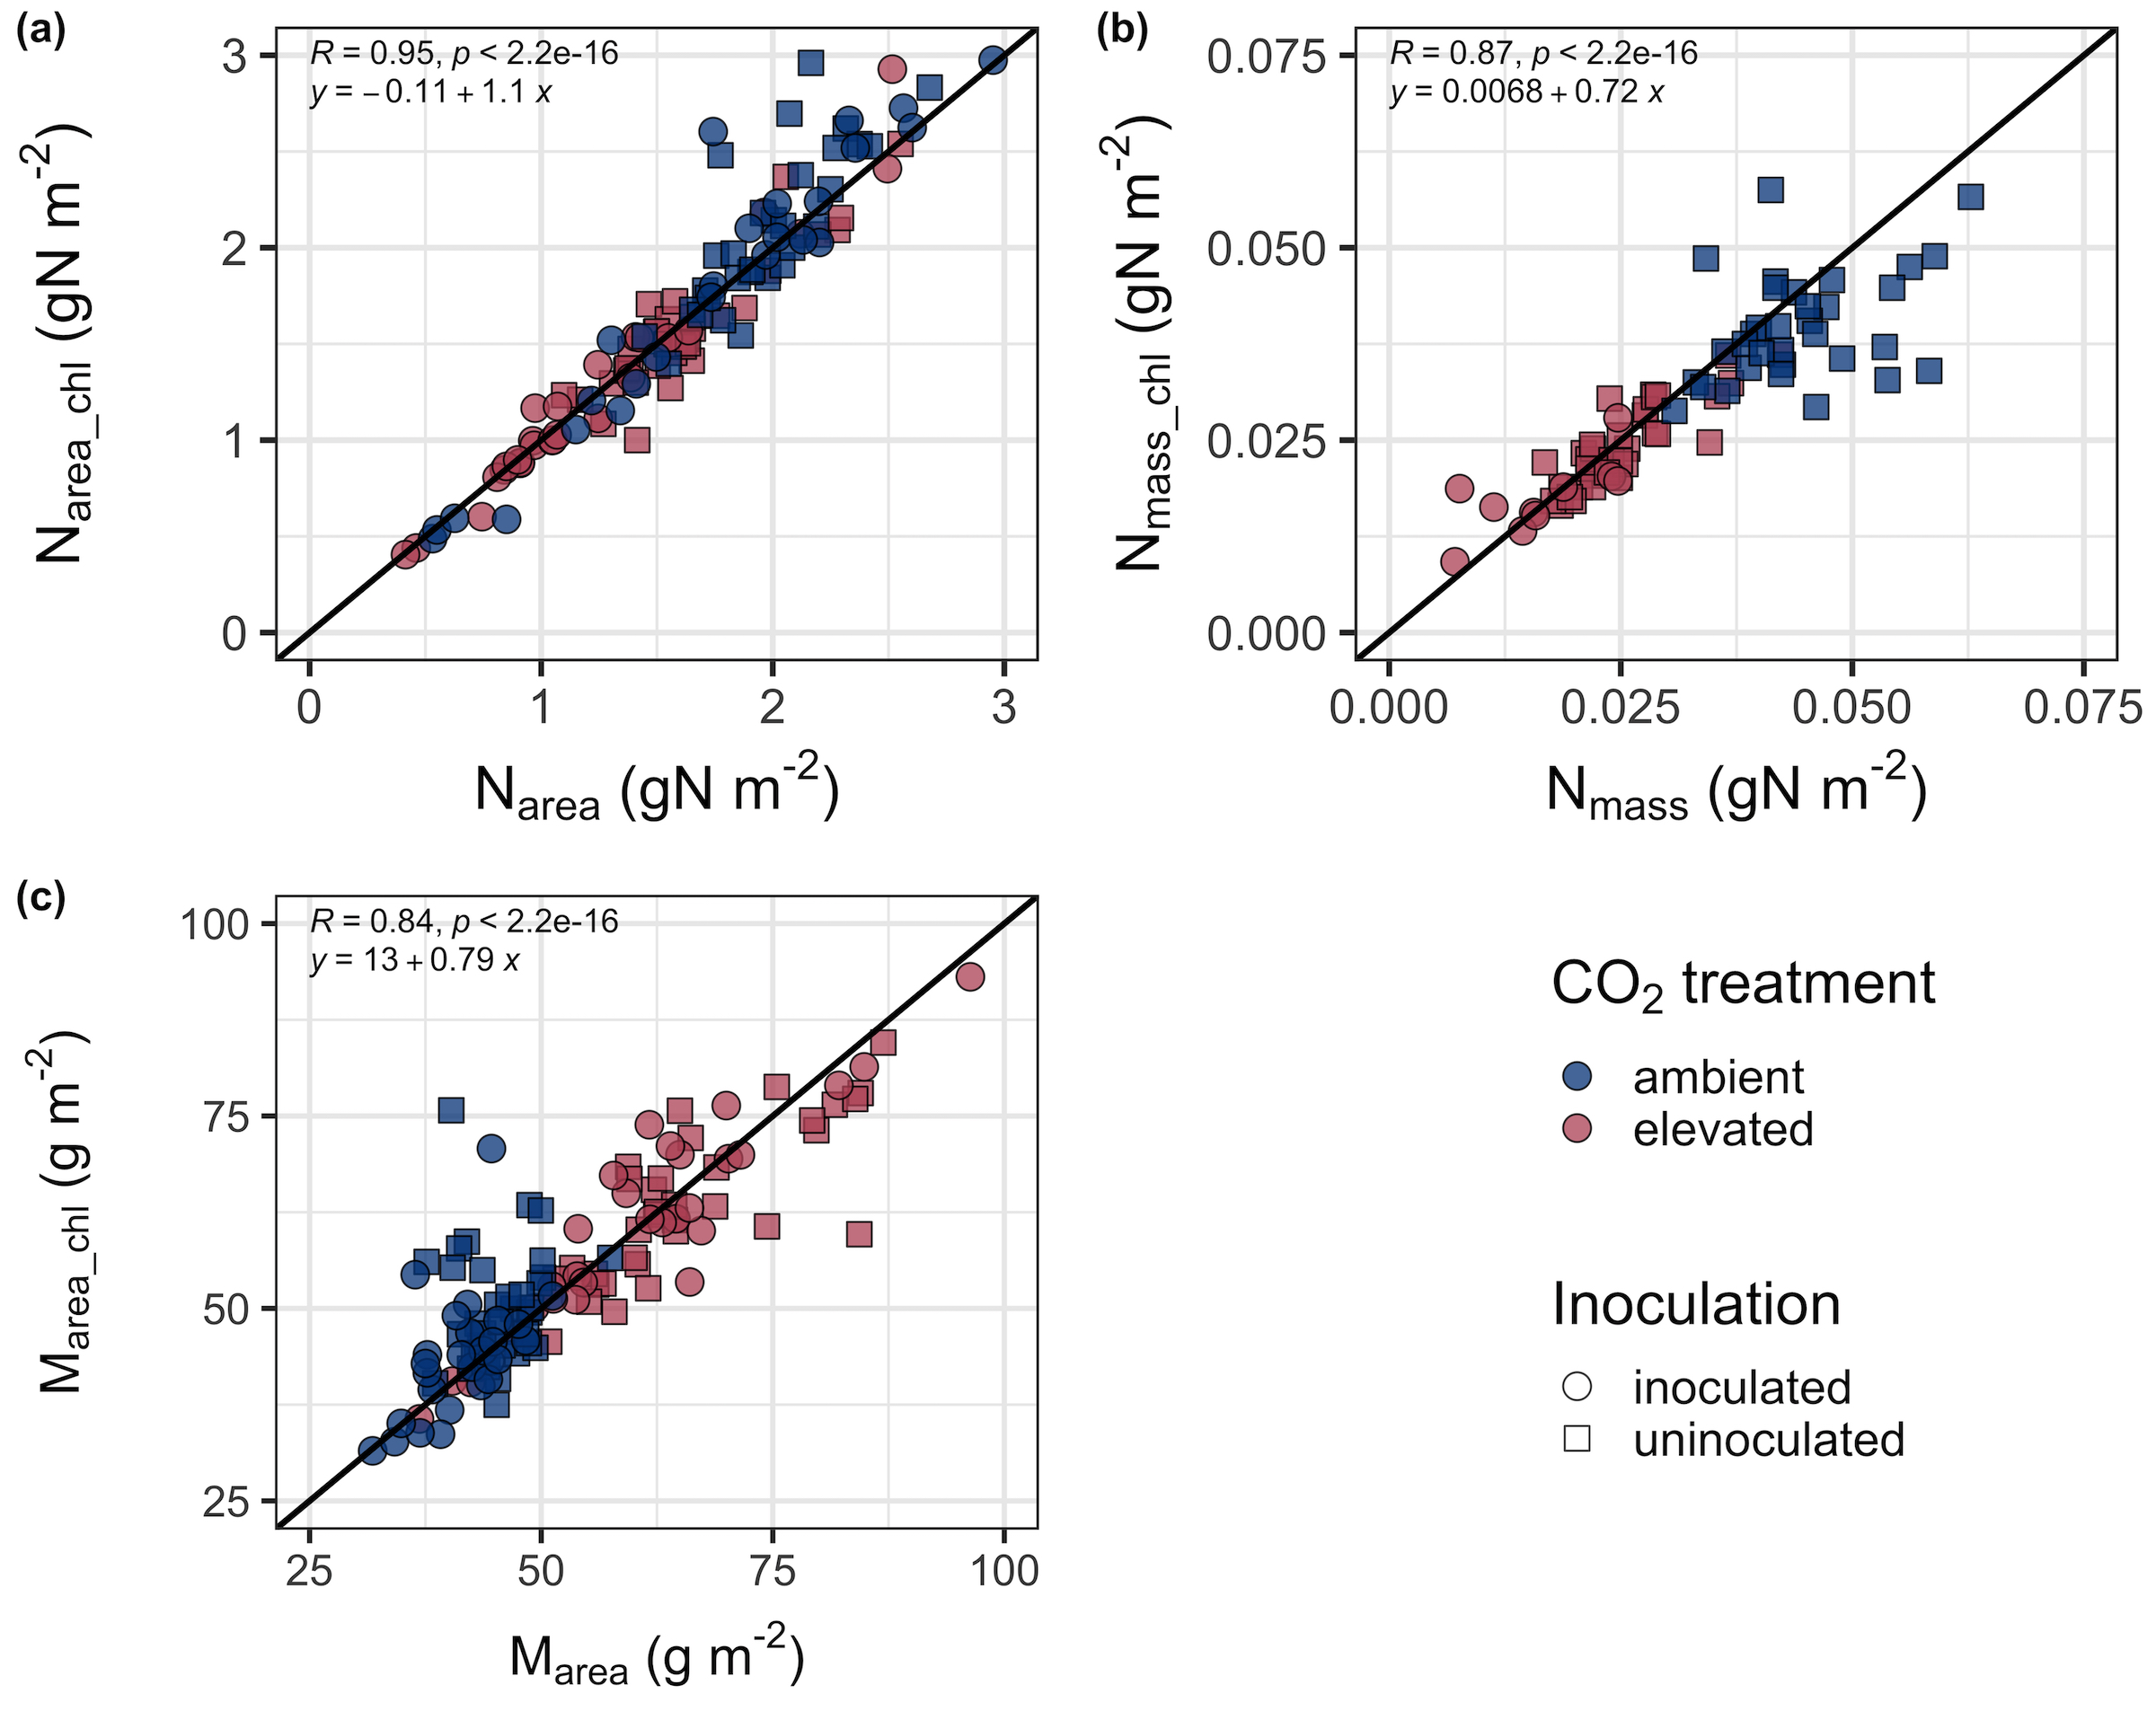
\includegraphics[width=\linewidth]{ch5_NxCO2xI/figs/NxCO2xI_figS1_leafN_chl.jpg}
    \caption[Relationships between area-based leaf nitrogen content, mass-based leaf nitrogen content, and leaf mass per unit leaf area measured on the focal leaf used to generate $A_\mathrm{net}$/$C_\mathrm{i}$ curves and leaf nitrogen content measured on the leaf used for chlorophyll extractions]{Relationships between area-based leaf nitrogen content (a), mass-based leaf nitrogen content (b), and leaf mass per unit leaf area (c) measured on the focal leaf used to generate $A_\mathrm{net}$/$C_\mathrm{i}$ curves (x-axis) and leaf nitrogen content measured on the leaf used for chlorophyll extractions (y-axis). Blue points refer to leaves grown under ambient CO$_2$ and red points refer leaves grown under elevated CO$_2$. Square points indicate uninoculated pots and circular points indicate inoculated pots. Pearson's correlation coefficient, associated \textit{p}-values, and the line of the regression line that described each bivariate are included in the top left corner of each plot. The solid black line visualizes the trend given a 1:1 bivariate relationship.}
    \label{fig:figure.d1}
\end{figure}
\clearpage

\newpage
\begin{figure}
    \centering
    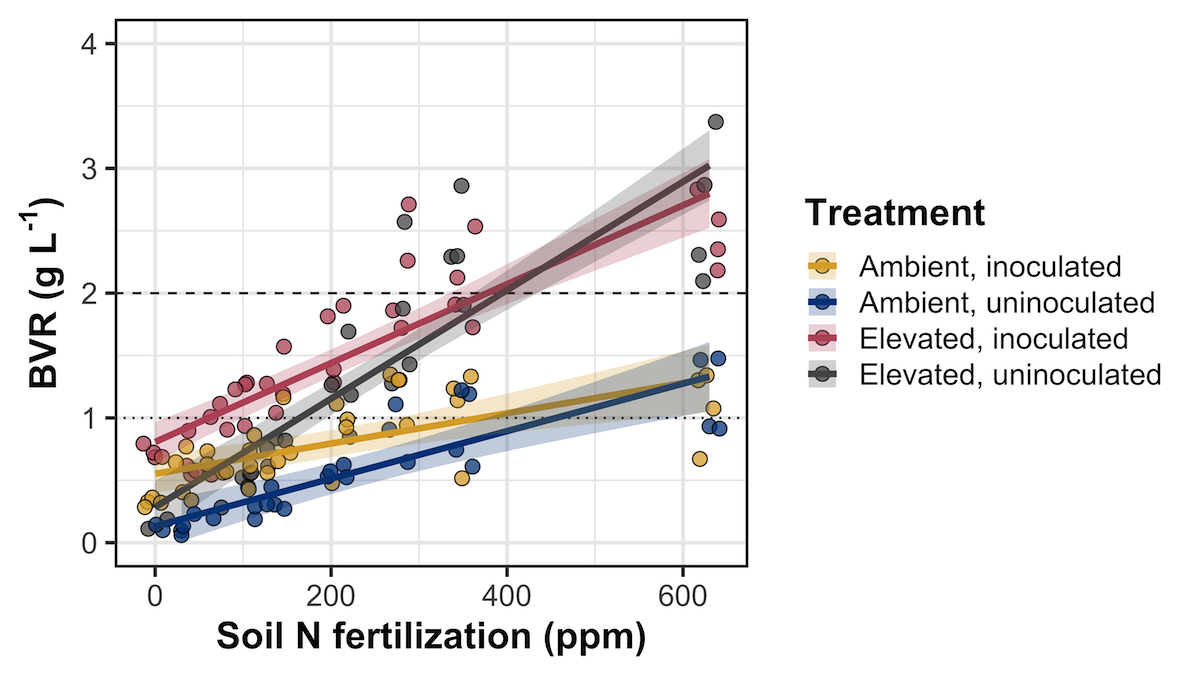
\includegraphics[width=\linewidth]{ch5_NxCO2xI/figs/NxCO2xI_figS2_bvr.jpg}
    \caption[Effects of CO$_2$, fertilization, and inoculation on the ratio of whole plant biomass to pot volume]{Effects of CO$_2$, fertilization, and inoculation on the ratio of whole plant biomass to pot volume. Soil nitrogen fertilization is represented on the x-axis in all panels. Yellow points and trendlines indicate inoculated individuals grown under ambient CO$_2$, blue points and trendlines indicate uninoculated individuals grown under ambient CO$_2$, red points and trendlines indicate inoculated individuals grown under elevated CO$_2$, and gray points indicate uninoculated individuals grown under elevated CO$_2$. Solid trendlines indicate regression slopes that are different from zero (\textit{p}<0.05). The dotted horizontal line indicates the point where biomass:pot volume exceeds 1 g L$^{-1}$, and the dashed line indicates the point where biomass:pot volume exceeds 2 g L$^{-1}$.}
    \label{fig:figure.d2}
\end{figure}
\clearpage
